\documentclass[sigconf, screen=true, nonacm]{acmart}

\usepackage{todonotes}
\setuptodonotes{size=\tiny}

\settopmatter{printacmref=false}
\setcopyright{none}
\renewcommand\footnotetextcopyrightpermission[1]{}

\hypersetup{pdftitle={Avail - Data Availability}}

\newcommand{\DA}{\textit{DA layer}}
\newcommand{\EX}{\textit{Exec layer}}
\newcommand{\DR}{\textit{DR layer}}

\begin{document}

\title{Avail: The Data Availability Blockchain}
\author{Avail \vspace{1cm}}

\begin{abstract}
    % We discuss a blockchain design where the data hosting and availability, contract execution and dispute resolution is decoupled. We further propose the details of the data layer which guarantees availability. 
    We study the scalability issue in present blockchain architecture and propose a design which decouples the data hosting, execution and verification. We discuss few suitable primitives for the construction of a data hosting layer that guarantees data availability. We sketch out the system goals, design, security and implementation details of Avail which is our availability focussed blockchain solution. 
\end{abstract}

\maketitle


\section{Present DApp Architecture}
    In present day Ethereum-like ecosystems, there are mainly three types of peers - validator nodes, full nodes and light clients. A block is appended to the blockchain by a validator node which collects transactions from the mempool, executes them, generates the block before propagating it across the network. The block contains a small block header containing digest and metadata related to the transactions included in the block. The full nodes across the network receive this block and verify its correctness by re-executing the transactions. The light clients only fetch the block header and fetch transaction details from neighbouring full nodes on an as-needed basis. The metadata inside the block header enables the light client to verify the authenticity of the received transactional details. 

    While this architecture is extremely secure and has been widely adopted, it has some serious practical limitations~\cite{Stanford:2020}. Because every transaction is executed by all the full nodes in the system, it becomes a bottleneck resulting in limited throughput. With wide adoption of such DApps, the number of transactions grow rapidly resulting in increased cost of including a transaction into a block. To counter these issues, layer 2 solutions have been proposed. 

    Layer 2 scaling solutions work by creating a chain anchored to the main chain like Ethereum. In such an architecture, DApps reside on the L2 chain and only periodic checkpoints are recorded on the main chain. The throughput in such a system depends on the transaction processing rate of the L2 chain whereas any dispute resolution can be performed on the main chain. The benefit of such a decoupled execution and dispute resolution is that it gives much higher throughput while retaining the security properties. In practice, multiple such L2 chains may function in parallel resulting in improved processing power of the system, while retaining the security of the main chain. 

\section{Plasma, Optimistic Rollup and ZK Rollup}\label{rollup}
    A major part of a successful layer 2 solution is the execution and verification framework. Plasma based sidechain approach can process thousands of transactions and submit only a single hash as checkpoint to the main chain. However, it faces an important issue. In case of a dispute on the sidechain, Plasma lacks an efficient mechanisms for users to exit the sidechain. Also, Plasma lacks the ability to process arbitrary instructions although they are supported by a quasi Turing-complete main chain like Ethereum. 

    Optimistic Rollups like Arbitrum and Optimism use the optimistic execution paradigm where a manager/operator executes the sidechain transactions and submits an assertion on the main chain. In case of dispute, other participants can challenge the assertion on chain within a fixed timeout and then the main chain performs the dispute resolution. While this scales up the transaction processing rate, it has a few downsides like delayed finality for non-fungible assets among others. 

    Zero-knowledge based rollups like Polygon zkEVM and Starkware take the ZK based approach to off-chain execution. The operators execute the transactions and submit a ZK proof to the main chain. The main chain can quickly verify the proof and on-chain participants can be assured that only valid state transitions were performed. 

    Another class of rollup is Validium which is a hybrid between Plasma and ZK based rollups. They make use of Zero-knowledge based proofs of execution and at the same time keep the transactional data off-chain. Although this improves the throughput of the system, they suffer similar problems to that of Plasma. User funds can be frozen or seized and other crypto-economic attacks are also possible on such a system. \cite{StarkEx:2020} provides a detailed discussion on the approach and possible attacks. 

    While there is still debate inside the community about which of these approaches is the best, we envision multiple such roll-ups operating simultaneously together forming the execution layer of our design. 

\section{The Data Availability Problem} 
    While the off-chain execution based architecture improves throughput, it is still limited by the amount of data that the main chain like Ethereum can handle. This is because although the execution is off-chain, the verification or dispute resolution is strictly on-chain. The transactional data is submitted as calldata on Ethereum to ensure that the data is available for future reconstruction. This is extremely important. In case of optimistic rollups, the operator may submit invalid transactions and then suppress parts of the block to the world. This way, the other full nodes in the system will not be able to verify whether the submitted assertion is correct. Due to lack of data, they will not be able to produce any fraud proof/challenge to show that the assertion is indeed invalid. In case of Zero-knowledge based rollups, the ZKP soundness ensures that accepted transactions are valid. However, even in the presence of such guarantees, not revealing the data backing a transaction can have serious side effects. It may lead to other validators not being able to calculate the current state of the system. \cite{EthWiki:2018} contains a detailed discussion on the subject. 

    We recognize that to achieve higher throughput, we not only need to put execution off-chain but also need to have a scalable data hosting layer that guarantees data availability. In later sections we discuss a design of such a decentralized Data Availability layer. 

\section{System Overview}
    \subsection{Decoupling the components}
        On a high level, a successful blockchain design needs to address the following components:
        \begin{itemize}
            \item \textbf{Data Hosting and Ordering:} This component would receive transactional data and order it without any execution. It would then store the data and ensure complete data availability in a decentralized manner. We call this component the \DA.
            \item \textbf{Execution:} The execution component should take ordered transactions from the \DA{} and execute them. It should create a checkpoint/assertion/proof and submit it to the \DR. We call this the \EX.
            \item \textbf{Verification/Dispute Resolution:} This component represents the settlement layer to which the system is anchored. The security of the design is dependent on the robustness and security properties of this component along with the \DA. The checkpoint or assertion or proof submitted by \EX{} is processed by this layer to guarantee that only valid state transitions are accepted in the system (provided that the data is available). We refer to this component as the \DR. 
        \end{itemize}

        In this work, we are proposing Avail, which acts as the \DA. We envision the multiple roll-up initiatives or legacy execution layers to form the \EX. The \DR{} can be any secure settlement layer which supports the execution verification.
    
    \subsection{Participants and System Goals}
        \subsubsection{Types of Nodes} 
            We consider the following types of nodes for Avail: 
            \begin{itemize}
                \item \textbf{Full Nodes:} The full nodes download the blocks and validate their correctness but do not participate in consensus. They store the blockchain but are not incentivized to participate or remain honest.
                \item \textbf{Validator Nodes:} The validator nodes take part in block generation and decide on transaction inclusion and ordering. These nodes are incentivized to participate in consensus and host the blockchain. Essentially, they are also full nodes with stake in the system. 
                \item \textbf{Light Clients:} These are clients with resource constraints who have access to only the block header and query transactional data from other full nodes on an as-needed basis. They want to have high confidence that the block is available, and when querying data they want a proof that the data belongs to the block. 
            \end{itemize}
            % We assume that the nodes are part of a peer-to-peer network with the light client connected to at least one honest full node. We have two types of adversaries in our system:
            % \begin{enumerate}
            %     \item \textbf{Ordering Attacker:} This type of adversary wants to disrupt the decentralized data hosting layer by either not allowing the blockchain to grow or by trying the network to accept two contradictory blocks. As our blockchain does not enforce any transactional logic but only enforces a strict ordering, the adversary of this type want to make the network accept two blocks with different orderings. We assume that at most $\frac{1}{3}$ of validators can be controlled by this adversary. 
            %     \item \textbf{Data Availability Attacker:} The DA attacker wants to hide a small portion of the data present inside a block and wants the network to accept such a block. We assume that majority of full nodes can go rogue and be controlled by this type of an adversary, but there is at least one honest full node with the entire data. We note that the DA attacker can target data present in any block and not just the most recent block. In particular, we want the \DA{} to be resistant against such an attacker for historical data as well. 
            % \end{enumerate}
        \subsubsection{System Goals}\label{goals}
            Our design for Avail should provide the following guarantees:
            \begin{enumerate}
                \item \label{goal:one} The decentralized data availability blockchain keeps producing a canonical chain of blocks even in the presence of an adversary that controls $<\!\!\frac{1}{3}$ of the validator nodes in the network. 
                \item \label{goal:two} The honest participants of the system with access to the canonical chain of block headers will not accept a block whose underlying data is unavailable even if a very powerful adversary is controlling all the other nodes in the system. Under the assumption that there are enough honest participants, the data should remain available for a limited amount of time. 
            \end{enumerate}
            We want to guarantee achieving both these system goals. We want to emphasize that both the goals have different adversarial assumptions. Goal \ref{goal:one} ensures that the blockchain system continues to function in a decentralized manner as long as a super-majority of validator nodes remain honest. Goal \ref{goal:two} ensures that an outside participant like an application running a light node, who has access to the canonical chain of block headers, need not trust any full node to have the guarantee that the underlying data for a particular block is available. This is an extremely strong assumption which eliminates any trust assumption to detect data hiding attempt. In the next sections we discuss our construction ideas and argue that they achieve these goals. 

\section{Designing the Data Availability Layer}
    \subsection{Primitives}
    %     Hash Function. Erasure Coding. Kate Commitment. \todo{expand}
        \subsubsection{Why is redundancy important in ensuring Data Availability?}
            Suppose we have a block $B$ divided into data chunks $D_1, \dots, D_n$. The block producer wants to suppress one chunk. Without loss of generality, let us assume that the first chunk is hidden by the block producer. Clients can query one chunk at random to get guarantees that data is indeed available. It can repeat this process many times so as to get sufficient confidence that the data is accessible. Hence, for each query, the block producer needs to be lucky enough that $D_1$ is not queried.

            However, with redundancy included by schemes like erasure coding, suppose the $n$ chunks are encoded into $2n$ chunks. Erasure coding ensures that any $n$ out of the $2n$ chunks are sufficient to recreate the data. This makes the hiding task harder for the block producer. To hide one particular chunk, it needs to make at least $n+1$ chunks unavailable. As a client, querying constant number of times gives a very high confidence that the data is indeed available. Hence, redundancy plays a vital role in the data availability. An erasure coding based design along with the related tradeoffs are discussed in \cite{albassam2019fraud}.

        \subsubsection{Fraud Proofs}
            In the previous section although we discussed the advantage of redundancy in data, we omitted the case when the erasure coded chunks are misconstructed by the block producer. In these cases, even though most chunks are indeed available, the entire block data might not be accessible. Hence, fraud proofs are constructed by other full nodes in the system and propagated to the light nodes. The light nodes verify the fraud proof and get convinced that the received block header is that of an erroneous block. An interesting property of fraud proofs is that they function even under a minority honest assumption. This is because having a single honest full node as a neighbour is sufficient for an honest light node to be guaranteed that it receives the fraud proof. 

            An important factor to consider during design of \DA{} is the size of fraud proofs. In simple erasure coded chunks, to proof that the encoding is incorrect, the entire original data block needs to be propagated to the light client. Hence, the fraud proof size is at least linear to the size of the block. Although we do not discuss the higher dimensional erasure coding based design here, we refer to \cite{albassam2019fraud} for a detailed analysis of fraud proof sizes. 

        \subsubsection{Commitment Size}
            In a one dimensional erasure coding based design, once a block producer selects data chunks $D_1, \dots, D_n$, it encodes the chunks to generate $D_1, \dots, D_{2n}$ (assuming coding rate to be $0.5$). It then constructs a Merkle tree over the chunks and keeps the root of it in the block header which acts as the commitment. A light client fetching $D_i$ gets a Merkle membership proof along with the data chunk so that it can quickly verify that a legitimate chunk has been supplied. The commitment (root of Merkle tree) size is an important factor to consider in any design. With large commitments, block headers become larger resulting in increased network traffic. While higher dimensional erasure coding based schemes achieve shorter fraud proof size, it comes at the cost of larger commitments. 

    \subsection{Coded Merkle Tree based Design}
        We briefly discuss the Coded Merkle Tree (CMT) based approach~\cite{yu2019coded} proposed by Yu \textit{et al.} The novelty of this approach is that it gives constant sized commitments with logarithmic sized fraud proofs. 

        The design uses systematic erasure codes at each layer of the Merkle tree. In particular, at the base layer, it takes $k$ data chunks and extends it to $n$ data chunks in such a manner that the first $k$ out of $n$ chunks are the original chunks and the rest are parity symbols. Each chunk in the next layer of the tree is made from hashes of $q$ chunks of the previous layer. Similar systematic erasure code is applied on that layer as well and we keep building successive levels of the tree until we have $t$ hashes which we keep as the commitment inside the block header. 

        When a light node samples a base layer chunk, the chunk along with a Merkle membership proof is given in such a manner that not only availability of base layer is ensured but also the higher layer availability is guaranteed. A light client sampling $s$ base layer chunks the Merkle membership proof will automatically sample $s$ intermediate layer chunks with high probability. 

        For a full client, decoding the tree and generation of fraud proof is also extremely efficient. With access to the root layer of the CMT present in the header and some coded chunks of the previous layer, the hash-aware peeling decoder decodes the previous layer getting access to all the hashes of the preceding layer. The decoder continues until all the chunks in the base layer is decoded or it finds evidence of an incorrect coding. In case of the former, the full node gets access to the entire data and in case of the latter, it generates the fraud proof and broadcasts it. 

        A detailed description of the construction along with performance analysis is present in \cite{yu2019coded}.

    \subsection{Kate Commitment based Design}
        In this section we first discuss polynomial commitments proposed by Kate \textit{et al.}~\cite{Kate:2010}. Then we go on to discuss a \DA{} design based on Kate commitments as proposed in \cite{EthResearch_DA:2020}. 

        Given a polynomial $\phi(x) \in \mathbb{Z}_p[x]$ over a bilinear pairing group, Kate \textit{et al.} proposed a scheme to have a commitment to the polynomial using a single group element. Moreover, the scheme supports opening of a commitment at a point $i$ to get $\phi(i)$ using constant sized witness that allows a verifier to confirm that $\phi(x)$ was indeed evaluated at $i$ to get $\phi(i)$. The commitment scheme is both computationally hiding and binding. The commitment scheme is additively homomorphic and supports a single witness for a batch of openings on multiple points of the same polynomial.
        
        Given such a scheme, the block producer breaks the block data into chunks such that each chunk is an element of the field. It arranges the chunks into n rows and m columns such that it forms an $n \times m$ matrix $D$. It uses the evaluation form to construct a polynomial from each row to obtain $\phi_1(x), \dots, \phi_n(x)$. It then commits each polynomial to get $C_1, \dots, C_n$ respectively. For redundancy, it extends $C_1, \dots, C_n$ to $C_1, \dots, C_{2n}$. It puts $C_1, \dots, C_{2n}$ inside the block header and broadcasts it. Figure \ref{fig:KC_data} shows the data arrangement and the corresponding commitments. 

        \begin{figure}[h]
            \centering
            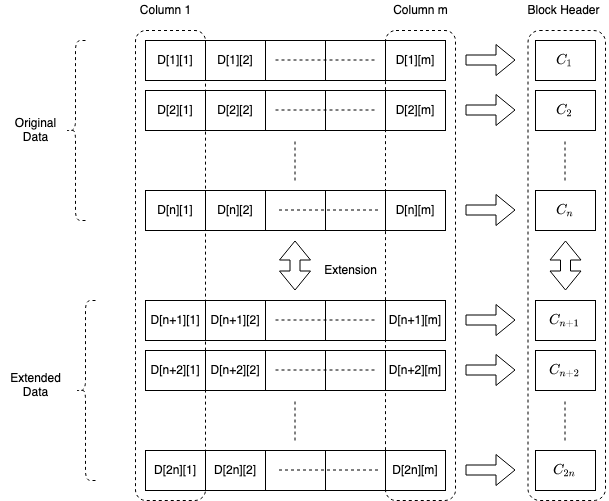
\includegraphics[width=\linewidth]{DA-KC-Data.png}
            \caption{Data Arrangement in Kate Commitment based \DA}
            \label{fig:KC_data}
        \end{figure}

        The light clients querying a data block will sample some chunk $D[i][j]$. Along with the data, the light client gets a witness $w[i][j]$ and it can immediately verify the validity using the Kate Commitment scheme discussed above. If it queries multiple chunks of the same row, the batch commitment scheme helps have a single witness for all the sampled points. Hence the membership proofs are extremely efficient. 

        For full nodes, the system can have two types of full nodes: 1. classical full nodes having entire block, 2. Column full nodes which keep only a single column of the data. For classical ones, it takes the entire matrix $D$, extends each column to $2n$ points and getting an extended matrix $D'$. 

        It then verifies for each row of $D'$ whether the commitment to $i^{th}$ row is $C_i$ for $1 \leq i \leq 2n$. 

        For the column full nodes, they can fetch and keep only a column of the matrix $D$. They would extend each column to check whether they belong to the extended set of commitments. This is possible because of the homomorphic nature of the commitments and witnesses. In particular, having $D[1][j], \dots,\allowbreak D[n][j]$ and $w[1][j],\allowbreak \dots, w[n][j]$, the node can extend both to $2n$ points and immediately verify whether the extended openings are valid. If the number of such column full node is $O(m)$, and each column full node ensures at least one column is available, then collaboratively the entire data is available within the column full nodes. 

        As the block size grows, so does the number of commitments (keeping number of columns fixed, the number of rows grow). Hence the commitment size grows linear to that of the block size. However, we do not need any fraud proofs in such a system. For each light client, the communication and computational overhead is constant. For each full node, the computational overhead is $O(m*n log(n))$ as it needs to perform $O(m)$ FFTs, $O(1)$ for each column, along with some pairing checks for verification. However, a column node has to only perform $O(n log(n))$ work because it works on a single column of data. 


\section{Analysis}
    \subsection{Attack Vectors}
        Any \DA{} needs to counter the following attacks on data availability:
        \begin{enumerate}
            \item \label{attack:ordering} A super-majority of the validators in the \DA{} wants to change the ordering of an already finalized block.
            \item \label{attack:wrong} A super-majority of the validators create a wrong block header, i.e., the commitment of the data present in the header is wrong. 
            \item \label{attack:hide} A super-majority of the validators want to hide at least one chunk of the block. For a light node, this would mean not being able to detect hiding of data with a non-negligible probability. For a full node, this would mean not being able to reconstruct the data. 
        \end{enumerate}

        We take the case of the super-majority of validators attacking the \DA{} because we want to minimize honesty assumption required for our design. 
        
        Under the assumption that finality is reached, the reordering attack (attack \ref{attack:ordering}) is hard to mount. This is because, to successfully mount this attack the attacker would need to break the non-equivocation property of the underlying consensus. In particular, the finality layer ensures that if equivocation occurs, the dishonest parties can be identified and their stake slashed. 

        In the subsequent sections we show how Attack \ref{attack:wrong} and Attack \ref{attack:hide} is countered in each of the two design choices - CMT and Kate Commitments.

    \subsection{Coded Merkle Trees}
        In the CMT based approach, the block proposer(s) may attempt to construct wrong header in two ways:
        \begin{itemize}
            \item The erasure coding in one or more layers is wrong. 
            \item The Merkle tree construction is wrong.
        \end{itemize}

        In both cases, the fraud proof captures such an attack. A full node, with access to the data, can build the incorrect-coding proof and broadcast it for the light clients. \cite{yu2019coded} contains a detailed description of such a fraud proof. 

        The random sampling from base layer by a light client also samples higher layers. As each layer is erasure coded, hence, probability of hiding any chunk from any of the layers of the Merkle tree is extremely low for sufficiently many samplings. A full client who wants to reconstruct the Merkle tree needs access to the block header which contains the root hashes. Along with that, it needs $(1-\alpha)n$ samples of the each layer, where $n$ is the total chunks in the layer and $\alpha$ is the minimum fraction of coded symbols a malicious block producer needs to make unavailable to prevent full decoding. With these information it can decode the entire tree. The entire decoding strategy along with the hash-aware peeling decoder construction is given in \cite{yu2019coded}. 

        Hence, the CMT approach can mitigate both attack \ref{attack:wrong} and \ref{attack:hide}.  We however note that the mitigation assumes a single honest full node, which is not as strong as Goal \ref{goal:two} defined in Section \ref{goals}. 

    \subsection{Kate Commitments}
        In the Kate commitment based approach, attack \ref{attack:wrong} amounts to a wrong commitment by the block producer. Without loss of generality, suppose $C_1$ is wrong. This would mean that at least one out of $D[1][1]$ to $D[1][n]$ does not belong to $C_1$. Again, let us assume $D[1][1] \not\in C_1$. This would mean that at least one of this is true: $D[n+1][1] \not\in C_{n+1}, \dots, D[2n][1] \not\in C_{2n}$. This is because $C_{n+1}, \dots, C_{2n}$ are extended from $C_1, \dots, C_n$ and $D[n+1][1], \dots, D[2n][1]$ are extended from $D[1][1], \dots, D[n][1]$. Hence, such an attack is caught by a light client with overwhelming probability. 

        In case of attack \ref{attack:hide}, a light client querying constant samples can achieve arbitrarily high confidence that the data is indeed available. This is due to the redundancy in the data as discussed previously. For a full node, it needs to download the at least $n$ chunks from each column so that it can reconstruct the entire extended data. It checks the commitments to know whether the downloaded data is correct. A column full node needs to perform similar operations but only for one column of data. Even if the supermajority wants to suppress data after some time, the light client P2P layer contains the data with redundancy. This enables new clients to recover block data without reliance on the full nodes or validators. 
        
        Hence, this approach mitigates all discussed attacks and achieves the goals set in Section \ref{goals}.
        
\section{Implementation}
    In this section, we discuss the implementation details of Avail. Among the two techniques discussed above, we use the Kate commitment based approach in order to avoid fraud proofs and provide strong data availability guarantees even in presence of powerful adversaries. 

    \subsection{Consensus}
        We need our validators to reach consensus on the next block which contains the ordered set of transactions along with redundant erasure coded data. 
        % To achieve that, we use a consensus protocol that satisfies the following:
        % \begin{itemize}
        %     \item \textbf{Safety:} No two honest nodes have finalized chain of blocks with two conflicting blocks. In our context, this means that all honest nodes agree on a unique ordering of transactions. 
        %     \item \textbf{Liveness:} Irrespective of previous events, new blocks can always be added to the chain and finalized. In our context, this ensures that new transactions are always added in the chain. 
        % \end{itemize} 
        Although there exists many possible blockchain consensus protocols, we opted for the  Proof-of-Stake (PoS) family of consensus algorithms. We wanted a PoS consensus that supports high number of validators, provable finality and a robust security framework. In particular, we chose the BABE/GRANDPA hybrid consensus used by Polkadot~\cite{polkadot_consensus:2020}. It uses two separate protocols for block production and finality.
        
        The block production is done using Blind Assignment for Blockchain Extension protocol (BABE)~\cite{BABE:2020}. The block producers produce blocks based on a Verifiable Random Function (VRF). The protocol does not assume access to a central clock. In case no validator is chosen as the block producer for a particular slot, or if the chosen producer(s) go down, there is a secondary block producer who can step in. BABE ensures liveness which guarantees that transactions submitted to honest players will eventually be inserted into the chain. 
        
        GRANDPA (GHOST-based Recursive ANcestor Deriving Prefix Agreement)~\cite{grandpa} is a finality gadget ensuring provable finality. Without the finality gadget, the users can only have probabilistic finality, like in classical blockchain systems. GRANDPA guarantees that blocks reach quicker finality and a finalized block can never be reverted. 

    \subsection{Full Nodes}
        To implement our design in a standalone blockchain, we use the Substrate framework~\footnote{https://github.com/paritytech/substrate}. Substrate provides great flexibility to implement custom runtime logic with inherent BABE/GRANDPA consensus support. Our design needed major changes in the Substrate codebase and hence we worked on a separate codebase~\footnote{https://github.com/availproject/avail}. The major changes that we made are:
        \begin{itemize}
            \item The contents of the block are arranged into the data matrix, extended and polynomial commitment generation is performed during the block building process. 
            \item The header structure is changed to contain the commitments as part of the header. 
            \item Block sizes are made dynamic, according to the number of transactions on the mempool. However, the maximum block size allowed is 4 MB, including the data redundancy.  
            \item Additional RPC methods to support data availability queries are introduced. These can be used by light clients to gain confidence about availability and inclusion.
        \end{itemize}
        We have modified the Polkadot Apps~\footnote{https://github.com/availproject/avail-apps} to build our block explorer~\footnote{https://testnet.avail.tools/} for our test network. 

    \subsection{Light Client}
        In our present design, light clients are nodes that participate in the system without investing resources to host a full node. We want our light clients to have very high data availability guarantees without hosting a full node or trusting on any other peer. Keeping this in mind, we have developed a light client~\footnote{https://github.com/availproject/avail-light} which keeps track of the chain header and performs availability queries to gain confidence on the availability of interested blocks. They also help contribute to data availability by hosting sampled data for other light clients within the P2P network. The client can gain as high confidence as deemed suitable for the specific application. We envisage the applications using our chain to host a light client.

    \subsection{Ethereum Data Availability Guarantees}
        A \DR{} layer like Ethereum, when validating proofs or resolving dispute, need assurance that the underlying data is indeed available (as discussed in Sec \ref{rollup}). To enable this in an organic manner, we want to guarantee data availability to a smart contract on Ethereum (or any settlement layer which supports this logic). This allows the checkpoint/assertion/proof accepting smart contract to communicate with this light client contract and directly get DA assurance. 

        We discuss three main approaches on how to provide the on-chain DA guarantee. We also briefly mention their advantages and limitations. 

        % \subsubsection{Light Client as a Smart Contract}
        %     The most obvious approach to achieve DA guarantee is to host the conventional light client as a smart contract. This provides the same guarantees on-chain as the off-chain light client. However, there are three main challenges to this approach:
        %     \begin{itemize}
        %         \item The smart contract needs a continuous feed of Avail chain headers. The primary concern is who submits these headers, how do we verify the submitted headers and how do we compensate the cost these submitting parties incur. We can take ideas from existing cross-chain bridging solutions to address these concerns. 
        %         \item The DA guarantee is highly dependent on the randomness of the queries. Smart contracts, on the other hand, can only run deterministic programs. We may use solutions like RANDAO~\footnote{https://github.com/randao/randao} to eliminate this bottleneck. 
        %         \item Even if the header is available to the contract, query is generated randomly and proof is submitted, the smart contract still needs to verify the responses to get confidence that the data is available. On-chain Kate commitment verification is challenging without supporting opcode for field operations. We could propose new pre-compiled contracts to support them but implementation requires consensus within the community and a hard fork.  
        %     \end{itemize}
        
        \subsubsection{Data Availability Oracle}
            A widely accepted approach for off-loading expensive tasks from smart contracts is the oracle based approach. When on-chain DA guarantee for a particular block is needed, multiple oracle nodes can be incentivized to submit their respective confidence factors. The on-chain contract can aggregate the metrics to decide whether it has sufficient guarantee that the data is available. Although well-accepted within the community, this approach has to trust the oracle nodes resulting in reduced security guarantees. The amount of trust can be limited by proper incentivization and decentralization. 

            \textbf{Proof of Concept Implementation}: To emphasize the viability of the protocol, we have implemented an on-chain light client using Chainlink Oracle Network, based on the second design discussed above. Whenever the on-chain contract needs availability guarantee for a particular block, it requests the on-chain Chainlink Oracle which uses events to communicate with multiple off-chain oracle nodes. These off-chain nodes use their own light clients or hosted instances to gain confidence and communicate the same back to the original contract through the Chainlink Oracle. The incentivization is handled using the LINK token. 

        \subsubsection{Bridges}
            A well-known approach for cross-chain message passing is using bridges. Using a bridge from Avail to \DR, the validators of Avail can attest to the fact that a particular piece of data is available. The downside of such approach is that it relies on the supermajority of the Avail validator set to be honest and to keep the data available. For most applications, this is a good enough assumption. 

            Under this model, the rollup operator submits the data on Avail and gets back a finalized block post transaction inclusion. It computes a proof of transaction inclusion within that block and posts it, along with proof of transactional validity, to the settlement rollup contract. The bridge operator(s), on the other hand, post finalized block metadata on the settlement layer. The rollup contract, upon receiving the proofs, checks the correctness of proofs against the bridge contract. The rollup transaction is accepted iff the proofs are verified to be correct. 
            
        % \subsubsection{Non-interactive DA proofs}
        %     The light client construction and security guarantees are based on an interactive protocol where the client queries to full nodes to get proofs which they verify to gain confidence on the availability. We need to explore making the protocol non-interactive where the light clients can subscribe to availability proofs without compromising the security. However, the guarantee that the data is available now does not enforce its availability in the future. We need to carefully design the protocol keeping security, efficiency and practicality in mind. 
        

\section{Additional Modules}
    \subsection{Application Specific Data Retrieval}
        We would want our construction to allow applications to download data which is only relevant to them. To enable this, we want the full nodes to prove to an application client that the complete set of data relevant to the application has been communicated.

        To enable Application Specific Data Retrieval (ASDR), we have introduced two main fields:
        \begin{itemize}
            \item \textbf{AppID}: Every transaction has been associated with an application identifier (appID). We envision rollup or application specific chains to register as applications if they want to download parts of block with only relevant application data. Any user is free to use the default appID `0' which is used for all types of transaction, including Avail system transactions. Any transaction with nonzero appID has to be of type application data submission only. 
            \item \textbf{appDataLookup}: Every block header contains an index field, containing the starting cell indices of application cells inside the block. This is created by the block producer when creating the block by grouping the data matrix by appID and then flattening it to infer the starting position of each group.  
        \end{itemize}

        The changes above together ensure that an application client can download only app-specific cells without downloading other application data.

        However, it is worth noting that there is no reliance on the block producer to create the index or group the data correctly. This is because, we create a deterministic algorithm that all honest application clients follow. Hence, all honest clients would retrieve the same app data for a particular appID. It can happen that clients get partial data, i.e., there exists data within the block associated with an appID which was not downloaded following the algorithm. However, the aim is to have the same view of their app to all honest app clients by providing them with same data. The polynomial commitments inside header assure that two clients with access to the same header cannot receive different sets of data. 

        % To illustrate, let us assume a roll-up \textit{R} operates on our proposed \DA. Hence, it would want to download only transactions which are intended for \textit{R}. 
        
        % For the CMT based approach, we can use a Namespaced Merkle Tree as described in \cite{lazyledger}. We would need to make some alterations to the original construction to make it work with the CMT. We leave the exact construction details for future work. 

        % For the Kate Commitment based approach, let us assume that each data chunk is prepended with an application identifier (ID) which is unique to the application. 
        % % For our example, let the ID for \textit{R} be $R$. 
        % Let the data matrix $D_{n \times m}$ be filled up column-wise and let the ordering be such that all transactions relevant to a particular application are put in contiguous chunks of data. Incomplete data chunks are padded appropriately. Let the application data be spread from $D[i_1][j_1]$ to $D[i_2][j_2]$, where $1 \leq i_1, i_2 \leq n$ and $1 \leq j_1 \leq j_2 \leq m$.   

        % With this setup, an application client can query its data from a full node. The full node need to give openings to all chunks from $D[i_1][j_1]$ to $D[i_2][j_2]$, taken column-wise. On top of that, it also needs to give openings to $D[i_1-1][j_1]$ (or $D[n][j_1-1]$ if $i_1=0$) and $D[i_2+1][j_2]$ (or $D[0][j_2+1]$ if $i_2=n$). The client can then verify that for all openings within $D[i_1][j_1]$ to $D[i_2][j_2]$, the data starts with the correct ID and for the remaining two openings, the data has a different ID. This would prove the client that it has received all relevant data, under the assumption that the ordering is done correctly (equivalently, that supermajority of validators are honest in \DA). 

        % In case the client approaches column full nodes, it would need to approach at most ($\lceil size/n \rceil + 2$) column full nodes. 
    

% \section{Related Work}
%     Lazyledger \cite{lazyledger} proposes a \DA{} construction using higher dimensional erasure coding. TODO: compare and contrast. 

% \section{Open Issues}
%     We note that a successful implementation of a \DA{} will need to address these issues:
%     \begin{itemize}
%         \item In Kate Commitment based scheme, a trusted setup phase is needed. A deeper look into the details of it is needed. Some representative numbers are present in \cite{dankrad_poly:2019}.
%         \item Aligning data chunks into field elements needs some engineering. Also, choosing a formally verified bilinear pairing library with high performance is critical. A good place to start would be blst library. 
%         \item Choice of parameters need to be carefully addressed. In CMT approach, the number of hashes in the root, coding rate, hashes per chunk, base layer data per chunk, etc., need to be chosen. In Kate commitment approach, the number of columns, choice of underlying group, etc., need to be fixed. In both approaches, simple parallelisation is possible which would increase efficiency. 
%     \end{itemize}

\bibliographystyle{ACM-Reference-Format}
\bibliography{DA_references}

\end{document}
